\documentclass{ExcelAtFIT}
%\documentclass[czech]{ExcelAtFIT} % when writing in CZECH
%\documentclass[slovak]{ExcelAtFIT} % when writing in SLOVAK


%--------------------------------------------------------
%--------------------------------------------------------
%	REVIEW vs. FINAL VERSION
%--------------------------------------------------------

%   LEAVE this line commented out for the REVIEW VERSIONS
%   UNCOMMENT this line to get the FINAL VERSION
%\ExcelFinalCopy


%--------------------------------------------------------
%--------------------------------------------------------
%	PDF CUSTOMIZATION
%--------------------------------------------------------

\hypersetup{
	pdftitle={Paper Title},
	pdfauthor={Author},
	pdfkeywords={Keyword1, Keyword2, Keyword3}
}

%--------------------------------------------------------
%--------------------------------------------------------
%	ARTICLE INFORMATION
%--------------------------------------------------------

\ExcelYear{2018}

\PaperTitle{Machine Translation Using Artificial Neural Networks}

\Authors{Jonáš Holcner*}
\affiliation{*%
  \href{mailto:xholcn01@stud.fit.vutbr.cz}{xholcn01@stud.fit.vutbr.cz},
  \textit{Faculty of Information Technology, Brno University of Technology}}

\Keywords{neural machine translation --- NMT --- recurrent neural networks --- RNN ---
LSTM --- encoder-decoder architecture --- sequence to sequence --- seq2seq ---
keras --- moses --- BLEU}

\Supplementary{\href{https://github.com/jojkos/neural-machine-translation}{Downloadable Library}}


%--------------------------------------------------------
%--------------------------------------------------------
%	ABSTRACT and TEASER
%--------------------------------------------------------

\Abstract{
The aim of this work is to develop a neural machine translation system (NMT). That is a machine translation system based on neural networks. Specifically, the system is based on the encoder-decoder architecture, created with recurrent neural networks enabling sequence to sequence translation.

The system is build with libraries Keras and Tensorflow and is tested against Moses statistical machine translation tool.

This work does not bring some concrete model with new state of the art results but shows some insight into the topic as well as provides an open source python library that can interested reader use to easily conduct his own experiments.
}

\Teaser{
	%\TeaserImage{teaser1.pdf}
	%\TeaserImage{teaser2.pdf}
	%\TeaserImage{teaser3.pdf}
    
\includegraphics[width=1\linewidth]{excelTeaser.pdf}
}

%--------------------------------------------------------

\begin{document}

\startdocument

%--------------------------------------------------------
%	ARTICLE CONTENTS
%--------------------------------------------------------

\section{Introduction}
In the recent years, there is a significant increase in usage of machine learning and artificial intelligence. This is because only lately, the capacity and performance of computers caught up with the available amount of data that is being produced every day as to build and train large enough neural networks. Now days, neural networks are widely capable of recognizing images, transcribing spoken language and most interestingly for this paper, they are quite capable in translating sequences from one language to another.

The biggest advantage of modern NMT approach is that it does not have some of the problems the traditional machine translation systems had. Instead of being composed of many different complex parts, NMT has the ability to learn and translate directly in end-to-end fashion.

Goal of this work is to develop and try out such system and provide an out of the box usable library. Solution proposed in this paper make use of the encoder-decoder architecture. Each of these two components is one recurrent neural network together capable of directly translating whole sequences from one language to another.

The result is python package \emph{nmt} built with Keras and Tensorflow. With this package were conducted experiments, evaluated with the standard BLEU score. Results were compared with the system produced by the Moses \cite{Moses} statistical machine tool.


\section{Previous Works}
First idea of recurrent neural networks comes from the nineties \cite{rnn}. The vanilla RNN, however, had a problem with long term dependencies because of the vanishing and exploding gradient \cite{gradientProblems}.

Thus came improved variants of the RNN -- long short term memory (LSTM) \cite{LSTM, forgetLSTM} and its simpler version, gated recurrent unit (GRU) \cite{GRU}. These units have a memory, that stores and changes information in it over time, enabling the network to remember long term dependencies.

Works \cite{neuralLanguageModels, neuralLanguageModels2, mikolovphd} shows that good performing language models are possible to build with recurrent neural networks. This lays foundation for the neural machine translation as language models are the vital part. The advantage of neural language model is that it learns embeddings in a continuous space for the words, which provides the model with more context it can learn from. Different variants of learning the word embbeddings are shown here \cite{word2vec,kingQueen,glove,fasttext}. Pre-trained word  embeddings, for example on some very large data set, can be used to boost performance of a NMT system, which would have to otherwise learn those embeddings by itself.

Encoder-decoder architecture was proposed in \cite{encoderDecoder} and was used for rescoring hypotheses produced by a phrase-based system with successful improvement. Paper \cite{seq2seq} then shows how to use encoder-decoder architecture for direct sequence to sequence translation and comes with the best results at the time. Furthermore, it was found that the importance of reversing order of the words  in all source sentences (reverse encoder), improves models performance, by introducing short term dependencies between the source and the target sentence.

Upon this builds work \cite{attention} which shows even better results with bi-directional encoder which is encoder that process in both normal and reverse order. What is even more important, they address the problem of encoder-decoder approach, where the meaning of the translated sentence is captured in a fixed-length vector and that can be problematic for translating long sentences. The proposed remedy is so called \emph{attention} mechanism which lets the model, at the time of decoding, look at the most important words from the source sentence for the currently translated word, resulting in even better performance.

As translation is an open-vocabulary problem, the NMT systems have to somehow handle the words not present at the time of the training. This was typically done by using out-of-vocabulary tokens and by using very large vocabularies, which causes the models to be very memory and performance demanding. Solution for this can be sub-word units \cite{mikolovSubwords, subwords}, that are shown to be more efficient, help with rare and unknown words and improve the results.

Current state-of-the-art results are published by Google \cite{googleBridgingGap,googleAttention}, which uses all of the techniques described, showing that they can be successfully applied on large production data sets.

Another thing Google shows is, that with no changes to the model architecture, one model can be used to learn to translate between many languages \cite{googleMultiLingual}, even to produce translations between languages that it was not explicitly trained on (zero-shot translations).

\section{Seq2seq translation with encoder-decoder architecture}
Sequence to sequence (\textbf{seq2seq}) means that the process of translating takes one whole sentence at the input, in a source language, and its meaning translates into sequence in a target language. This can be better in contrast to other methods like word-based translation or phrase-based translation as in seq2seq the whole meaning of the source sequence is translated at once and can keep the precise meaning. Seq2seq is modeling probability of a target sentence based on source sentence as shown in figure \ref{fig:seqProbability}.

\begin{figure}[h!]
    \begin{center}
        \setlength{\fboxsep}{8pt}
        \fbox{$W_{in}$ = ``Ahoj světe"}
        $\Longrightarrow$
        \fbox{$W_{out}$ = ``Hello world"}
    \end{center}
	\caption{Seq2seq models a probability $P(W_{out}|W_{in})$. Meaning that the model learns to predict sentence $W_{out}$ based on a sentence $W_{in}$.}
	\label{fig:seqProbability}
\end{figure}

Neural network architecture, used for this kind of modeling, is \textbf{encoder-decoder}. Both encoder and decoder are recurrent neural network (figure \ref{fig:rnn}), usually one or more layers of LSTM or GRU.

\begin{figure}[h!]\centering
  \centering
  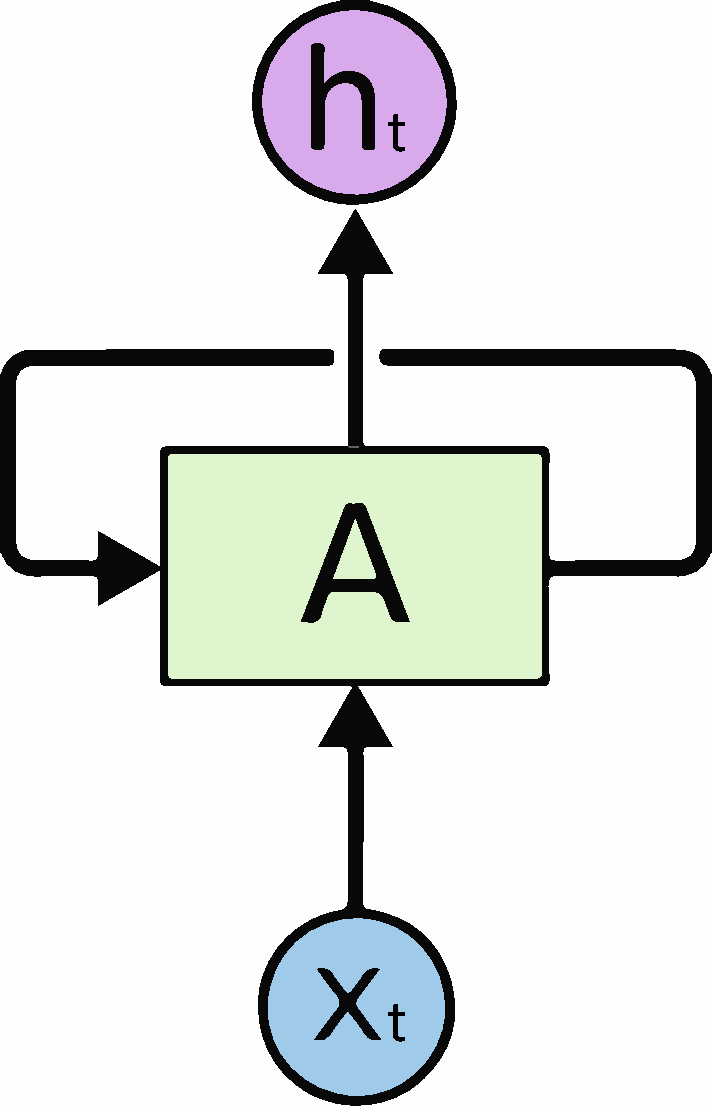
\includegraphics[width=0.5\linewidth]{RNN-rolled}
  \caption{RNN are neural networks with loops. They process sequence of data and output $h_t$ from each time step $t$ is fed as input to time step $t+1$. Image taken from \cite{understandingLSTM}.}
  \label{fig:rnn}
\end{figure}


Encoder takes embeddings of the input tokens (words or subwords) and processes the input sequence in source language into fixed-length vector, so called ``thought" vector -- it captures the essence of the given sentence.

Decoders hidden state is initialized with this output from encoder. The decoding process is started with start token, which is given to decoder as first input. Decoder then generates sequence in target language until it reaches end token that tells it to stop. There is a difference between time when model is being trained and between time when it is used to predict sequences. In the training time, decoder is fed the correct, expected output. This is called ``teacher forcing" \cite{teacherForcing}. In the inference time, decoder is fed its own output each time step. Figure \ref{fig:seq2seq} shows the encoder-decoder architecture.

\begin{figure*}[h!]\centering % Using \begin{figure*} makes the figure take up the entire width of the page
  \centering
  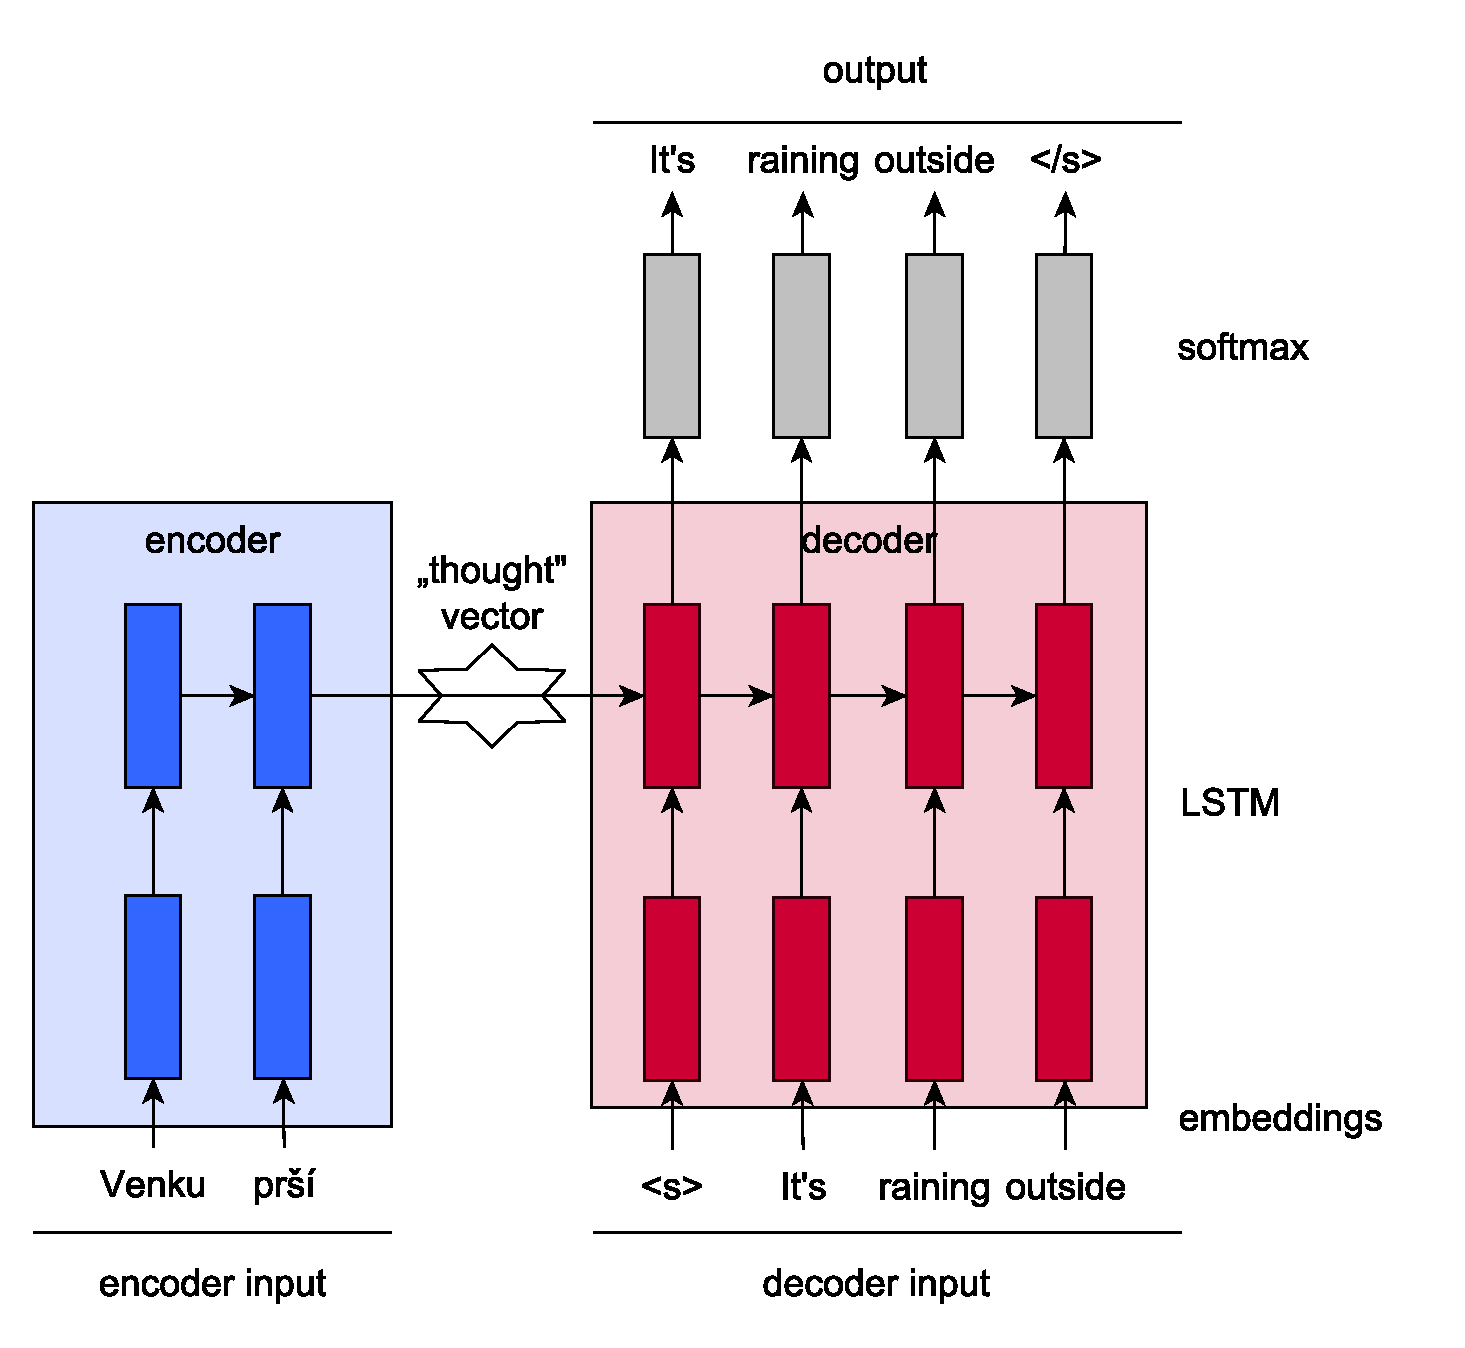
\includegraphics[width=0.82\linewidth]{seq2seqEn.pdf}\\[1pt]
  \caption{Encoder-decoder architecture shown on translation from Czech sentence to its English equivalent. Encoder processes embeddings of input sequence and produces fixed-length ``thought" vector. This vector is used as initial state of decoder, it tells it from what context should it produce output in target language. Prediction is started with the $\langle s \rangle$ starting token. Then the decoder is fed either correct output tokens during training time or its own output, from time $t - 1$, during inference time, until it generates the ending $\langle /s \rangle$ token.}
  \label{fig:seq2seq}
\end{figure*}

\hfill \break
Equations of the encoder-decoder architecture:
\begin{linenomath}
\begin{align}
    m^{(f)}_{t}&=M^{(f)}_{f_t}\label{figure:encoderEmb} \\
    h^{f}_{t}&=\begin{cases}
                    RNN^{(f)}(m^{(f)}_{t},h^{(f)}_{t-1}) & \mbox{if t $\geq$ 1},\label{figure:encoderState} \\
                    0 & \mbox{otherwise}.
                \end{cases}\\
    m^{(e)}_{t}&=M^{(e)}_{e_{t-1}}\label{figure:decoderEmb} \\
    h^{e}_{t}&=\begin{cases}
                    RNN^{(e)}(m^{(e)}_{t},h^{(e)}_{t-1}) & \mbox{if t $\geq$ 1},\\
                    h^{f}_{|F|} & \mbox{otherwise}.
                \end{cases}\label{figure:decoderState} \\
    p^{(e)}_{t}&=\mbox{softmax}(W_{hs}h^{(e)}_{t} + b_{s}) \label{figure:resultSoftmax}
\end{align}
\end{linenomath}

\begin{itemize}
    \item $RNN^(f)$ - encoder, $RNN^(e)$ - decoder
    \item $M^{(f)}_{f_t}$ - embedding for encoder input in time $t$
    \item $M^{(e)}_{e_t}$ - embedding for decoder input in time $t$
    \item $h^{(f)}_t$ - encoder hidden state in time $t$
    \item $h^{(e)}_t$ - encoder hidden state in time $t$
    \item $W_{hs}$ - weights
    \item $b_s$ - bias
\end{itemize}


Embedding is looked up for every word in time $t$ (eq. \ref{figure:encoderEmb}). Then the hidden state of encoder is computed (eq. \ref{figure:encoderState}). After processing the whole input sequence, there should be enough context stored for decoder initialisation. Then, as for encoder, embedding is looked up for decoder input (eq. \ref{figure:decoderEmb}). Only now the word is from time $t - 1$ as decoder generates new word based on the last one. In the time $t_0$ decoder is fed starting symbol $\langle s \rangle$. Eq. \ref{figure:decoderState} computes hidden state of decoder and shows that in the time $t_0$, decoder is initialised with encoder final state. Final output probability is resolved with $softmax$ function (eq. \ref{figure:resultSoftmax}).

For a deeper overview of NMT based systems, I would point the reader to \cite{nmtTutorial}.

\section{Implementation of the NMT system}


datasets
preprocessing
bucketing
fit generator?
bidirectional encoder
subwords - BPE
beam search
shuffling
main.py repo


\begin{figure*}[h!]\centering
  \centering
  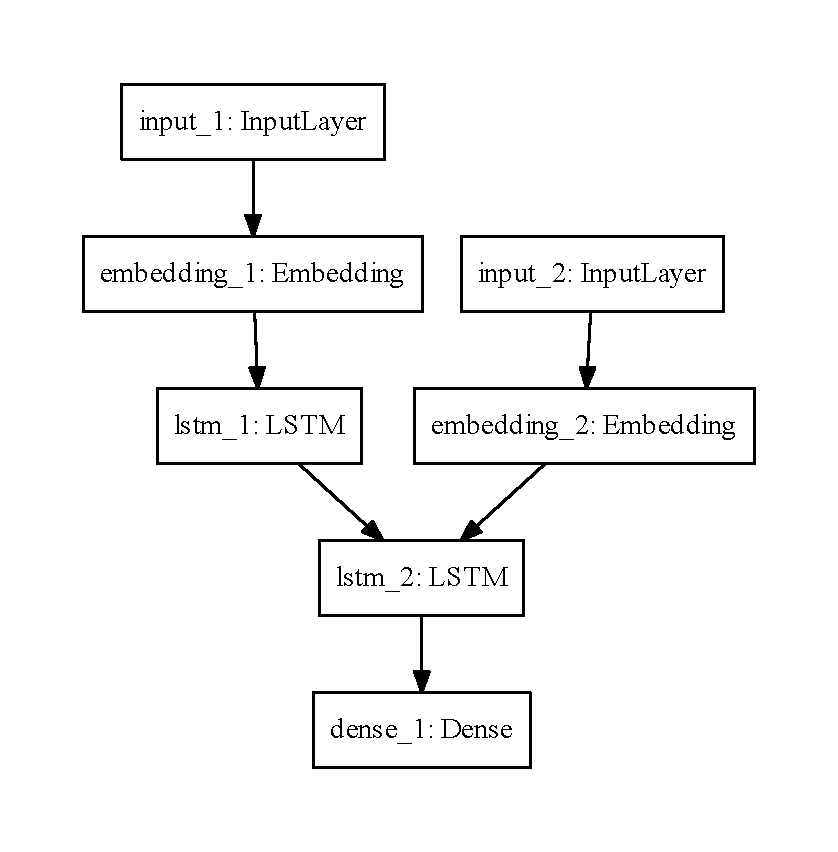
\includegraphics[width=1\linewidth]{model}
  \caption{Layers of model in keras}
  \label{fig:model}
\end{figure*}

\section{Experiments and results}

\section{Conclusions}
\label{sec:Conclusions}

\textbf{[Paper Summary]} What was the paper about, then? What the reader needs to remember about it?

\textbf{[Highlights of Results]} Exact numbers. Remind the reader that the paper matters.


\textbf{[Paper Contributions]} What is the original contribution of this work? Two or three thoughts that one should definitely take home.


\textbf{[Future Work]} How can other researchers / developers make use of the results of this work?  Do you have further plans with this work? Or anybody else?


\section*{Acknowledgements}
I would like to thank my supervisor Ing.~Igor Szőke,~Ph.D. for his help.


%--------------------------------------------------------
%	REFERENCE LIST
%--------------------------------------------------------
\phantomsection
\bibliographystyle{unsrt}
\bibliography{2018-ExcelFIT-NeuralMachineTranslation}

%--------------------------------------------------------
%--------------------------------------------------------
%--------------------------------------------------------
\end{document} 